\documentclass[journal]{IEEEtran}

\usepackage{cite}
\usepackage{amsmath,amssymb,amsfonts}
\usepackage{graphicx}
\usepackage{booktabs}
\usepackage{array}
\usepackage{url}
\usepackage{hyperref}
\hypersetup{hidelinks}
\usepackage{tikz}
\usetikzlibrary{arrows.meta,positioning,fit,backgrounds}
\tikzset{
  box/.style={draw, rounded corners=2pt, font=\footnotesize, align=center,
              inner sep=3pt, minimum height=6.5mm, line width=0.6pt},
  lbl/.style={font=\scriptsize, fill=white, inner sep=1.2pt, align=center},
  arr/.style={->, >=Stealth, line width=0.6pt},
  var/.style={draw, circle, font=\scriptsize, minimum size=7mm, inner sep=0pt, line width=0.6pt},
  fac/.style={draw, fill=black!75, minimum size=2.6mm, inner sep=0pt},
}

% Figures already tracked in the repository, plus this report's own.
\graphicspath{{figures/}{../../docs/images/hud/}{../../docs/images/vr-pipeline/}}

\newcommand{\code}[1]{\texttt{#1}}

\markboth{DeepGIS Technical Report, November 2026}%
{Das: DeepGIS: A Language-Driven Geospatial Platform with a Spatiotemporal World Model}

\begin{document}

\title{DeepGIS: A Language-Driven Geospatial Platform\\
with a Spatiotemporal World Model,\\
Live Robots, and Immersive Exploration}

\author{Jnaneshwar~Das%
\thanks{J.~Das is with the Earth Innovation Hub and the DREAMS Lab, School of Earth and Space
Exploration, Arizona State University, Tempe, AZ, USA (e-mail: jdas@earthinnovationhub.org).}%
\thanks{Technical report, version of 23 November 2026. It describes the system deployed at
\url{https://deepgis.org} and the open-source code at
\url{https://github.com/Earth-Innovation-Hub/deepgis-xr}. Unless stated otherwise, the results are
single runs on the live system or in simulation, not rates.}}

\maketitle

\begin{abstract}
DeepGIS is a web geospatial platform that puts a 3D globe of the Earth, the Moon and ten other
planetary bodies, open-vocabulary vision models, live robots and their digital twins, and an
immersive virtual-reality cockpit behind one plain-language interface. A user types or says a
request such as ``fly to Yuma at 8000\,m and show NDVI'' or ``what changed here since April?''.
A language model chooses from a fixed catalogue of typed actions. The server validates and clamps
every field. The page runs the plan on the same camera controls a person uses. Actions that
command a robot, build a simulation or change stored beliefs are only proposals, and a person
confirms them. This report describes the architecture and its main subsystems.
The central technical contribution is a spatiotemporal world model. Each capture of the globe
is turned into a scene graph by fusing several detectors under one urban taxonomy, and stored
as evidence in a bitemporal factor graph in PostGIS. Every world object carries a category variable
and an existence chain. Category beliefs come from local loopy belief propagation over perceptual,
geometric, contextual and feedback factors. Existence beliefs come from hit and miss evidence that
decays toward ignorance with a category-specific half-life. Misses count only where the capture
could have resolved the object. The store holds 103 captures, 46{,}121 detections and about
241{,}000 active factors. We report what building it taught us: a world model makes a detector's
errors durable unless its confidence is calibrated, uncertainty is shown, and nothing is ever erased.
\end{abstract}

\begin{IEEEkeywords}
Geographic information systems, digital twins, factor graphs, scene graphs, belief propagation,
large language models, human--robot interaction, open-vocabulary segmentation, WebXR, field robotics
\end{IEEEkeywords}

%======================================================================
\section{Introduction}
\label{sec:intro}

\IEEEPARstart{F}{ield} science and field robotics share one loop. Robots and people collect
observations. The observations are stored, looked at, annotated and modelled. The models go back
to the robots as maps, targets and behaviours. Each leg of that loop usually has its own tool:
a desktop GIS for maps, a notebook for detections, a ground station per vehicle, and a simulator
whose terrain was built by hand. The joins between those tools are where most of the effort goes.

DeepGIS puts the legs of the loop behind one surface: a browser globe that anyone can open at
\url{https://deepgis.org}. The design goals are:
\begin{enumerate}
\item \emph{One interface for every body and every task.} The same heads-up display (HUD), camera
drone and AI pilot work on the Earth, the Moon and the planets. The same requests drive data
layers, detectors, robots, twins and the world model.
\item \emph{Language as a planner, not as an actuator.} A language model chooses typed actions and
numbers. The server keeps only known types and fields and clamps every number. The page executes
the plan on existing controls. Anything with consequences outside the page is a proposal that
a person confirms.
\item \emph{Memory with honest uncertainty.} Detections are evidence about persistent world
objects, not facts. The store keeps every observation with the time it held and the time it was
recorded, never erases, and reports how sure it is.
\item \emph{Robots and twins in the same picture.} Field robots and simulated twins report pose and
camera frames to the same globe, and the pilot can follow, describe and (for authorised users)
command them.
\end{enumerate}

This report describes the system as deployed in November 2026: the architecture
(Section~\ref{sec:arch}), the viewer and its data layers (Section~\ref{sec:viewer}), the AI pilot
(Section~\ref{sec:pilot}), viewport perception (Section~\ref{sec:perception}), the spatiotemporal
world model (Section~\ref{sec:world}) and the pilot's questions over it
(Section~\ref{sec:worldpilot}), live vehicles and digital twins (Section~\ref{sec:robots}), and the
immersive cockpit (Section~\ref{sec:vr}). Section~\ref{sec:practice} covers how the system is
built and operated, and Section~\ref{sec:limits} what is still missing.

%======================================================================
\section{Related Work}
\label{sec:related}

\emph{Decision-support systems.} DeepGIS grows out of the lab's earlier work on data-driven
robotic sampling for ocean monitoring~\cite{das2015ijrr}, structure from motion combined with
deep learning for geomorphology~\cite{chen2020iros}, rock trait distributions mapped from drone
surveys of fault scarps~\cite{chen2023espl} and the OpenUAV cloud testbed~\cite{anand2019openuav}. The globe
is CesiumJS~\cite{cesium}; the novelty is not the renderer but what sits behind it.

\emph{Open-vocabulary perception.} Segment Anything~\cite{kirillov2023sam} made class-agnostic
masks cheap; SAM~3~\cite{carion2025sam3} adds segmentation by text concept. Grounding
DINO~\cite{liu2024gdino} detects boxes from text. Mask R-CNN~\cite{he2017maskrcnn} remains
useful for a fixed class trained on lab data. DeepGIS runs these as remote services and treats
each as a \emph{source} with its own confusion model rather than as ground truth.

\emph{Scene graphs and factor graphs.} 3D scene graphs~\cite{armeni2019sg} organise a scene into
objects and relations; Kimera~\cite{rosinol2021kimera} and Hydra~\cite{hughes2022hydra} build them
in real time from SLAM, with layers from places to buildings. Factor graphs~\cite{kschischang2001,
dellaert2017} are the common language for such estimation, and loopy belief
propagation~\cite{murphy1999loopy} is the usual approximate inference for discrete variables.
Existence modelling with a hit/miss sensor model follows occupancy grids~\cite{moravec1985}.
DeepGIS borrows the hierarchy and the pose-anchored evidence of Kimera but works at city scale from
globe imagery, stores the graph bitemporally~\cite{snodgrass1999}, and infers locally on demand.

\emph{Language models and robots.} SayCan~\cite{ahn2022saycan} and Code as
Policies~\cite{liang2023cap} ground language in robot skills. DeepGIS takes the narrower position
of a constrained JSON schema over typed actions, with the server as the gate, reached through the
Model Context Protocol~\cite{mcp2024}.

%======================================================================
\section{System Architecture}
\label{sec:arch}

\begin{figure}[t]
\centering
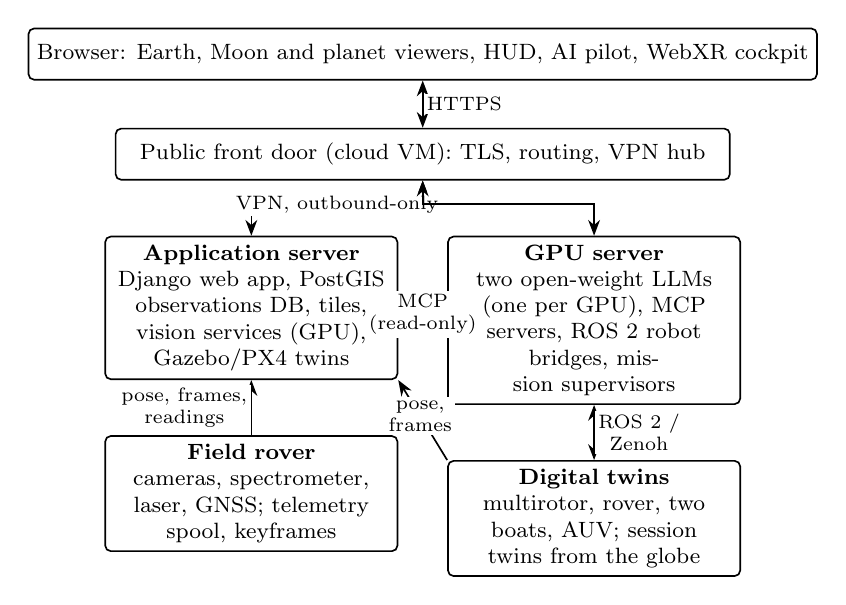
\begin{tikzpicture}[node distance=5mm and 4mm]
\node[box, minimum width=78mm] (browser) {Browser: Earth, Moon and planet viewers, HUD, AI pilot, WebXR cockpit};
\node[box, below=6mm of browser, minimum width=78mm] (edge) {Public front door (cloud VM): TLS, routing, VPN hub};
\node[box, below left=7mm and -36mm of edge, minimum width=37mm, text width=35mm] (app)
  {\textbf{Application server}\\Django web app, PostGIS\\observations DB, tiles,\\vision services (GPU),\\Gazebo/PX4 twins};
\node[box, below right=7mm and -36mm of edge, minimum width=37mm, text width=35mm] (gpu)
  {\textbf{GPU server}\\two open-weight LLMs\\(one per GPU), MCP\\servers, ROS~2 robot\\bridges, mission supervisors};
\node[box, below=7mm of app, minimum width=37mm, text width=35mm] (rover)
  {\textbf{Field rover}\\cameras, spectrometer,\\laser, GNSS; telemetry\\spool, keyframes};
\node[box, below=7mm of gpu, minimum width=37mm, text width=35mm] (twins)
  {\textbf{Digital twins}\\multirotor, rover, two\\boats, AUV; session\\twins from the globe};
\draw[arr, <->] (browser) -- node[lbl, right]{HTTPS} (edge);
\draw[arr, <->] (edge.south) -- ++(0,-3mm) -| node[lbl, pos=0.25]{VPN, outbound-only} (app.north);
\draw[arr, <->] (edge.south) -- ++(0,-3mm) -| (gpu.north);
\draw[arr, <->] (app) -- node[lbl]{MCP\\(read-only)} (gpu);
\draw[arr] (rover) -- node[lbl, left]{pose, frames,\\readings} (app);
\draw[arr, <->] (twins) -- node[lbl, right]{ROS 2 /\\Zenoh} (gpu);
\draw[arr] (twins.north west) -- node[lbl, pos=0.55]{pose,\\frames} (app.south east);
\end{tikzpicture}
\caption{DeepGIS by role. The only public entry is a small cloud VM; lab machines open outbound
VPN tunnels to it and accept no inbound connections. Network addresses are deliberately omitted.}
\label{fig:arch}
\end{figure}

Fig.~\ref{fig:arch} shows the system by role. The constraints that shaped it are practical. The lab
runs its own domain and accepts no inbound connections, so a small cloud VM terminates TLS, routes
requests and is the hub of a hub-and-spoke WireGuard network; lab machines dial out to it. A
round trip over that overlay is around 100--200\,ms and jittery, so nothing that needs a control
loop runs across it: autonomy stays on the robot, and the network carries plans, poses, frames
and batched data.

The \emph{application server} runs the Django~5.2 web application (gunicorn in Docker, with the
checkout bind-mounted), a PostGIS observations database for the world model and stored field
readings, a vector/raster tile server, the vision services on a second GPU, and the Gazebo/PX4
digital twins. The \emph{GPU server} keeps two open-weight language models resident, one per GPU
(a 26\,B mixture-of-experts Gemma model as the default and a 27\,B Qwen model with vision),
behind two Model Context Protocol (MCP) servers: a read-only one that the web application uses, and
a command-enabled one for robot commands. It also runs the ROS~2 language bridges and mission
supervisors for each robot. The registry database is SQLite; the observations database is the
only PostgreSQL instance, routed by a Django database router so that no long read can lock the
registry.

The web code base has about 43{,}000 lines of Python and 9{,}100 lines of HUD JavaScript, 252 test
methods in 23 files, and 381 commits since December 2024.

%======================================================================
\section{The Viewer and its Data Layers}
\label{sec:viewer}

\begin{figure}[t]
\centering
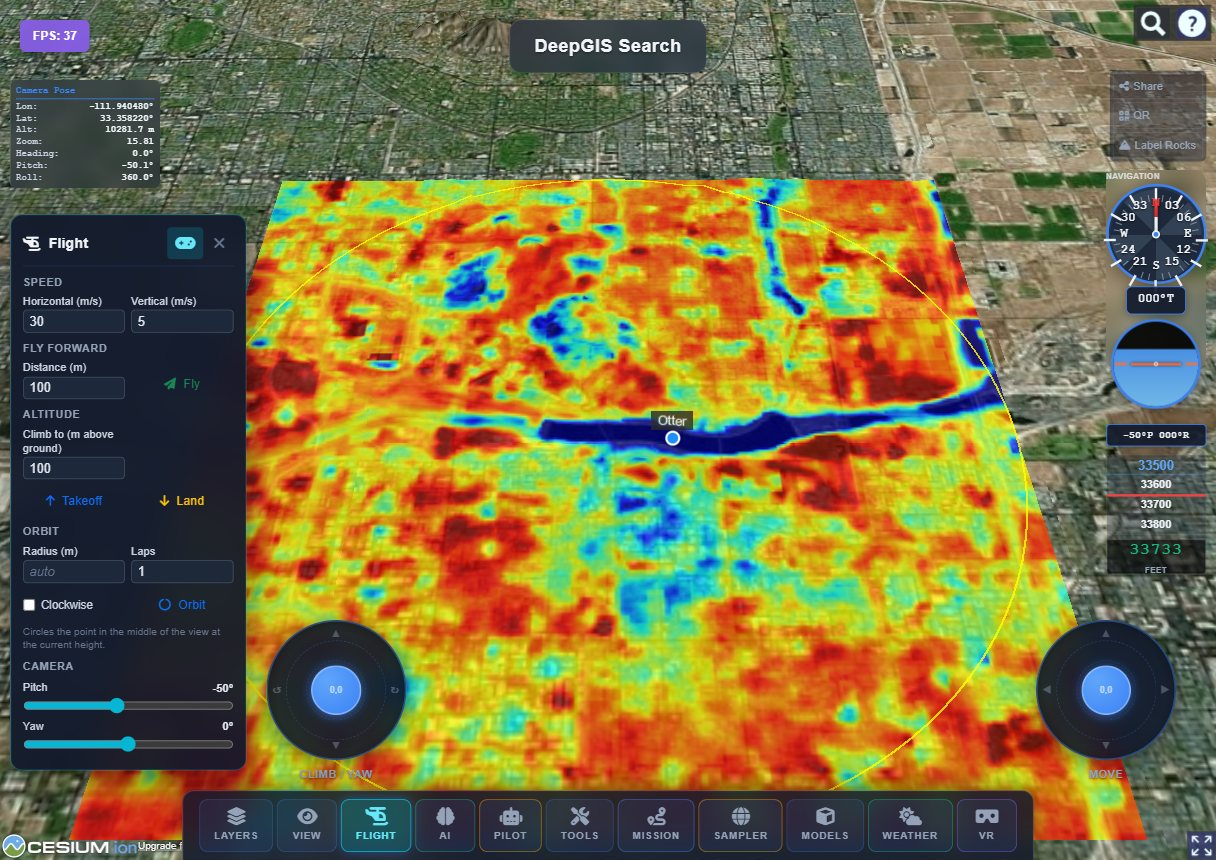
\includegraphics[width=\columnwidth]{hud-flight-panel.jpg}
\caption{The Earth viewer: Landsat~9 surface temperature within 5\,km of Tempe Town Lake, the
Flight panel, virtual joysticks, the camera pose and the toolbar. The pin is a boat twin's live
position.}
\label{fig:hud}
\end{figure}

Every viewer shares one HUD (Fig.~\ref{fig:hud}): a toolbar, a camera drone with speed, fly-forward,
takeoff, land and orbit controls, virtual joysticks, a layers panel and the AI pilot chat. The page
opens in 2D; any action that needs heading or tilt switches to 3D instantly, because Cesium's
animated morph ends at a fixed whole-globe camera and loses the view.

On Earth the pilot and the layers panel offer 24 layer kinds in groups: geology (Macrostrat),
Quaternary faults, flood, fires, rivers, land cover, soils, wildlife, trails, springs, mines,
surface temperature, NDVI, humidity, air and sea temperature, chlorophyll, elevation, slope,
contours, lidar elevation models, topographic datasets, and the lab's own survey imagery and
features. Rasters are fetched from their public sources and coloured in the browser with a named
colour map; vector features are drawn with their attributes and sources listed in the chat. The
lab's tile catalog serves drone orthophotos down to 0.68\,cm per pixel and vector layers such as
222{,}657 segmented rock outlines at a fault-scarp site; because Cesium~1.111 has no vector-tile
support, vector tiles are rendered server-side to styled PNG tiles, and a small decoder answers
point queries against them. The Moon and planet viewers use the same HUD with planetary imagery,
terrain-derived layers and the IAU gazetteer for place names.

%======================================================================
\section{The AI Pilot}
\label{sec:pilot}

\subsection{From a sentence to a checked plan}
A request goes from the page to \code{POST /label/api/pilot/} with the message, the body being
viewed, the current view (centre, altitude, heading, pitch, activity) and recent chat history. The
server adds context lines that the model needs and cannot see: named places near the view, the
live robots with distance and bearing, the 3D models placed nearby, the available models, and
today's date. It then calls the language model through the read-only MCP server with a JSON
schema for \code{\{reply, actions\}}.

The reply is not trusted. \code{clean\_actions} keeps only known action types; for each type it
keeps only that type's fields, clamps every number to a per-field range, resolves place names
(curated geology sites, then the robot registry, then a geocoder), drops bad coordinates, and
reorders steps where the order matters (a layer is drawn before an orbit starts). A plan that
promises an action but contains none is retried once. The page then runs the plan on the
same controls a person uses. Plans are cancellable: a new request or Stop interrupts the current
plan. \emph{Passive} actions (layers, describing the view, the world-model questions) do not stop
a running orbit or follow.

\begin{table}[t]
\caption{Pilot action types on Earth}
\label{tab:actions}
\centering
\footnotesize
\begin{tabular}{@{}>{\raggedright\arraybackslash}p{33mm}>{\raggedright\arraybackslash}p{51mm}@{}}
\toprule
Action & What the page does \\
\midrule
\code{goto}, \code{orbit}, \code{adjust} & fly to a place; orbit it (optionally until stopped); retune a running orbit \\
\code{takeoff}, \code{land}, \code{look},\newline\code{stop}, \code{wait} & camera-drone motion \\
\code{show\_layer}, \code{hide\_layer} & draw or remove one of 24 data layers \\
\code{place\_model} & stand a catalogued 3D model on the terrain \\
\code{describe\_view}, \code{check\_view} & vision model on the frame; check a goal for the view \\
\code{follow\_vehicle} & ride a live robot's camera or chase it \\
\code{find\_objects} & SAM~3 on the view: outlines, counts, area histogram \\
\code{show\_scene\_graphs} & stored captures and the world model in view \\
\code{world\_uncertain},\newline\code{world\_confidence},\newline\code{capture\_quality},\newline\code{world\_changes} & questions over the world model (Section~\ref{sec:worldpilot}) \\
\midrule
\code{robot\_command}$^\ast$ & propose a command for a robot (confirm card) \\
\code{create\_twin}$^\ast$ & build a Gazebo twin of the view (confirm card) \\
\code{retire\_entity}$^\ast$ & retire the selected world object (confirm, undo) \\
\bottomrule
\multicolumn{2}{@{}p{84mm}@{}}{\scriptsize $^\ast$Superusers only: offered in their schema and prompt, dropped by the server for anyone else.}
\end{tabular}
\end{table}

Table~\ref{tab:actions} lists the 20 action types every signed-in user can get on Earth and the
three that only superusers can. Off Earth the catalogue shrinks to motion, layers that exist for
that body, models and the vision actions.

\subsection{Long-form tasks}
A plan that ends in \code{check\_view} carries a goal for the view (``the inside of the crater is
visible''). After the plan runs, the vision model compares the frame with the goal and returns
\code{\{met, seen, suggestion\}}. When the goal is not met, the chat sends a ``goal check'' turn
back to the planner with what was seen, up to three rounds. While an orbit is running,
\code{adjust} retunes its radius, altitude, pitch or speed without restarting it.

\subsection{Propose, clamp, confirm}
Three actions have consequences beyond the page. \code{robot\_command} proposes a command for a
robot; the chat shows it as a card and nothing is sent until the user presses Send, which goes to
the command-enabled MCP server under the user's identity. \code{create\_twin} proposes a Gazebo
world of the ground under the crosshair (Section~\ref{sec:robots}). \code{retire\_entity}
proposes taking a world object out of the world model. The web application holds only the
read-only MCP token, so the language path itself cannot command a vehicle. The pattern
recurs across the system and we adopt it as a principle: language models propose, rules clamp,
humans confirm, and fast loops stay on the robot.

Typical latency is about 3\,s with a warm model and up to 40\,s after the model has been idle.

%======================================================================
\section{Viewport Perception}
\label{sec:perception}

The AI panel and the pilot's \code{find\_objects} send the current frame to remote vision services:
SAM, Grounding DINO~\cite{liu2024gdino}, a Mask R-CNN~\cite{he2017maskrcnn} trained on rock
outlines, and an Ultralytics service~\cite{ultralytics} that serves YOLO26, open-vocabulary
YOLOE-26 and SAM~3~\cite{carion2025sam3}. Models load per request and unload afterwards so that
one 11\,GB card serves them all next to a simulator. Results are drawn on the globe from the frame's
ground footprint. When a service is down the endpoint returns an empty, explicitly
\emph{degraded} result instead of an error, so plans continue.

Two engineering details mattered more than any model choice. First, the corners of the footprint
must be picked on the terrain, not the ellipsoid: a fallback to the ellipsoid at the top row of the
canvas stretched every overlay north at a site 350\,m above it. Second, the capture must exclude the
system's own overlays. Until this was fixed, a rebuild sent the models an image with our previous
polygons painted on it, and their output was stored as new evidence. We now hide every result
layer during capture: what the system believes must not reach it as observation.

Observed behaviour at nadir over Tempe: YOLO-family models trained on ground-level imagery found
almost nothing but cars; Grounding DINO found buildings and trees; SAM~3 found 86 cars with masks
about 1.5--2 times a car's area (median 18.6\,m$^2$), because neighbouring cars merge at the
service's input resolution.

%======================================================================
\section{A Spatiotemporal World Model}
\label{sec:world}

\subsection{From a capture to a scene graph}
A \emph{capture} is one frame of the globe with its ground footprint, camera pose, time and pixel
size. A scene-graph build runs the selected sources on it (SAM~3 with editable text prompts, YOLO,
Grounding DINO, plain SAM, and others) and fuses their claims into nodes under one taxonomy,
\code{urban\_v1}, with 14 categories: building, house, solar panel, road, vehicle, pavement, parking
lot, tree, other vegetation, bare ground, water, pool, debris and unknown. Each source $s$ has a
confusion table $Q_s(\ell \mid c)$, the probability that it reports native label $\ell$ for an
object of category $c$. Text-prompted sources get tables built from prompt--category affinities,
with a catch-all for unmatched prompts. Fusion~\cite{kernelcal} combines the claims that overlap
into one node with a category posterior and links nodes by adjacency and containment.

\subsection{The store}
The scene graph is then ingested into a PostGIS store (tables \code{sg\_*}): captures, poses,
kernel runs, detections, the claims behind them, \emph{entities} (persistent world objects with a
cached posterior, existence probability, geometry, first and last sighting), associations,
factors, belief snapshots and user feedback. Factors are \emph{bitemporal}: each has the interval
in which it holds, the time it was recorded, and the time it was superseded, if ever. Nothing is
deleted. A correction or a better rule supersedes the old factor at one instant, so the belief at
any past time and the belief as it was known at any past time can both be recomputed.

\subsection{The factor graph}
\begin{figure}[t]
\centering
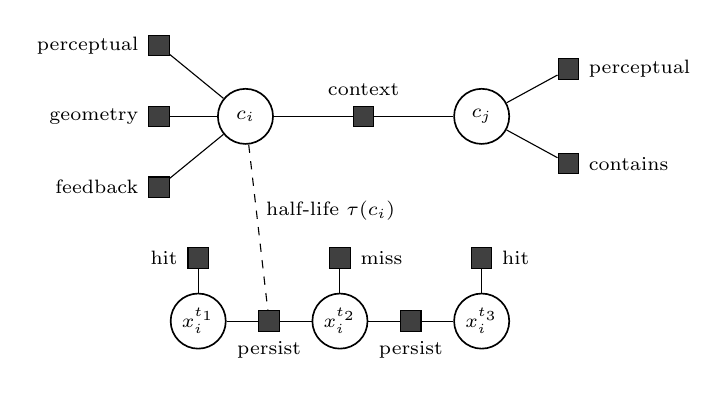
\begin{tikzpicture}[x=10mm,y=10mm]
\node[var] (ci) at (0,0) {$c_i$};
\node[var] (cj) at (3,0) {$c_j$};
\node[fac, label={[font=\scriptsize]above:context}] (fij) at (1.5,0) {};
\draw (ci) -- (fij) -- (cj);
\node[fac, label={[font=\scriptsize]left:perceptual}] (p1) at (-1.1,0.9) {};
\node[fac, label={[font=\scriptsize]left:geometry}] (g1) at (-1.1,0) {};
\node[fac, label={[font=\scriptsize]left:feedback}] (fb) at (-1.1,-0.9) {};
\draw (ci) -- (p1); \draw (ci) -- (g1); \draw (ci) -- (fb);
\node[fac, label={[font=\scriptsize]right:perceptual}] (p2) at (4.1,0.6) {};
\node[fac, label={[font=\scriptsize]right:contains}] (k2) at (4.1,-0.6) {};
\draw (cj) -- (p2); \draw (cj) -- (k2);
\node[var] (x1) at (-0.6,-2.6) {$x_i^{t_1}$};
\node[var] (x2) at (1.2,-2.6) {$x_i^{t_2}$};
\node[var] (x3) at (3.0,-2.6) {$x_i^{t_3}$};
\node[fac, label={[font=\scriptsize]below:persist}] (t12) at (0.3,-2.6) {};
\node[fac, label={[font=\scriptsize]below:persist}] (t23) at (2.1,-2.6) {};
\draw (x1) -- (t12) -- (x2) -- (t23) -- (x3);
\node[fac, label={[font=\scriptsize]left:hit}] (h1) at (-0.6,-1.8) {};
\node[fac, label={[font=\scriptsize]right:miss}] (m2) at (1.2,-1.8) {};
\node[fac, label={[font=\scriptsize]right:hit}] (h3) at (3.0,-1.8) {};
\draw (x1) -- (h1); \draw (x2) -- (m2); \draw (x3) -- (h3);
\draw[dashed] (ci) -- node[pos=0.4, right, font=\scriptsize]{half-life $\tau(c_i)$} (t12);
\end{tikzpicture}
\caption{The factor graph of two entities. Each entity $i$ has a static category variable $c_i$
and an existence chain $x_i^{t}$ at the times it was observed or missed. Persistence factors are
derived at query time from a half-life that depends on the category.}
\label{fig:fg}
\end{figure}

Each entity $i$ has a static category variable $c_i$ over the taxonomy and a binary existence
variable $x_i^t$ at each time it was observed (Fig.~\ref{fig:fg}). The category factors are:
\begin{itemize}
\item \emph{perceptual}: $\log Q_s(\ell \mid c_i)$ for each claim, down-weighted by age with a
five-year half-life;
\item \emph{geometry}: a plausibility term on the detection's ground area $A$,
\begin{equation}
g(c, A) = \max\!\Big(\phi,\; -\kappa \max\big(0,\, \ln\tfrac{A_{\min}(c)}{A},\, \ln\tfrac{A}{A_{\max}(c)}\big)\Big),
\label{eq:geom}
\end{equation}
with $\kappa = 2$ per e-fold outside the plausible range $[A_{\min}, A_{\max}]$ (a vehicle
1.5--120\,m$^2$, a house 30--3{,}000\,m$^2$) and floor $\phi=-8$; a road region larger than
5{,}000\,m$^2$ with compactness $4\pi A/P^2 \ge 0.35$ is a frame-clipped blob, not a road, and gets
$-3$. Unknown is unconstrained, so an implausible region drifts toward unknown rather than
becoming a giant car;
\item \emph{context}: a symmetric co-occurrence table between adjacent entities (a vehicle next to a
parking lot $+0.7$, a pool next to a road $-0.5$), at most six neighbours each;
\item \emph{contains}: a parent--child table (a solar panel on a house $+1$, a vehicle inside a
building $-1$);
\item \emph{feedback}: a user's confirmation or relabelling, worth about four observations.
\end{itemize}

The existence chain has \emph{hit} and \emph{miss} factors with $P(\text{detected}\mid
\text{present}) = 0.8$ and $P(\text{detected}\mid\text{absent}) = 0.05$, linked by persistence
factors that forget toward ignorance:
\begin{equation}
P(x^{t'} = x^{t}) = \tfrac12 \big(1 + 2^{-(t'-t)/\tau(c)}\big),
\label{eq:persist}
\end{equation}
where the half-life $\tau(c)$ is 4\,h for a vehicle, 30 days for debris and unknown regions, one year
for other vegetation, two years for a tree and five years for buildings and roads. A car is an
event; a building is a fact. These transitions are derived at query time from the category
belief, never stored.

A miss is recorded only when the capture's footprint covers at least 90\% of the entity, a source
that has seen it before ran on this capture, and the entity is large enough to resolve:
\begin{equation}
A_i \ge N_{\min}\, \mathrm{GSD}^2, \qquad \mathrm{GSD} = \sqrt{A_{\text{footprint}} / N_{\text{pixels}}},
\label{eq:miss}
\end{equation}
with $N_{\min} = 64$ pixels. Applying this rule to the stored evidence superseded 14{,}793 misses
that a coarse capture could never have turned into a sighting. A detection that covers more than
half the footprint is the frame itself (a whole-image box or a smeared mask): it is stored and
gated, but never becomes evidence.

\subsection{Association and inference}
A new detection joins an existing entity when their polygons overlap with IoU $\ge 0.3$, or, for
similar-sized small objects whose masks jitter between captures, when their centroids are within
2\,m. Otherwise it creates an entity. Inference is local: after an ingest, loopy belief
propagation with damping 0.5 runs over the category variables of the touched entities only, with
their neighbours held as fixed boundary priors, and an exact forward filter computes each
existence chain. The vectorised BP matches a reference factor-graph implementation to $10^{-6}$ in
the tests. A 69-node capture ingests in about 1\,s plus 0.1\,s of BP. Passing a time $t$ recomputes
every belief as of $t$, which is how the panel offers ``as it was then''.

An entity whose top category probability is below 0.25 is labelled \emph{unknown} and keeps its
best guess. The threshold sits in the valley of the stored score distribution: most unlabelled
regions (plain SAM masks, untyped map polygons) are nearly uniform over the taxonomy, at 0.10 to
0.20, and the next mode is at 0.30 to 0.35.

\begin{table}[t]
\caption{World-model state, 23 November 2026}
\label{tab:world}
\centering
\footnotesize
\begin{tabular}{@{}lr@{\hspace{6mm}}lr@{}}
\toprule
\multicolumn{2}{@{}l}{Evidence} & \multicolumn{2}{l@{}}{Entities (lon/lat)} \\
\midrule
Captures (Apr--Nov 2026) & 103 & unknown & 14{,}507 \\
Detections & 46{,}121 & building & 6{,}153 \\
Perceptual factors & 46{,}121 & house & 284 \\
Hit factors & 46{,}121 & road & 244 \\
Miss factors (active) & 5{,}922 & pavement & 185 \\
Miss factors (superseded) & 14{,}793 & tree & 142 \\
Context factors & 112{,}200 & vehicle & 135 \\
Contains factors & 2{,}451 & other vegetation & 102 \\
Geometry factors & 28{,}069 & pool, lot, solar & 112 \\
\midrule
GSD 5/50/95th pct.\ & \multicolumn{3}{l@{}}{0.13 / 0.57 / 2.48\,m per pixel} \\
\bottomrule
\end{tabular}
\end{table}

Table~\ref{tab:world} gives the current state. A further 16{,}749 entities from 24 captures in
April 2026 have projected metres stored as degrees (a replay bug); they are excluded from every view
and await reprojection.

\subsection{What the data taught us}
The first version of the store was a lesson in how a memory amplifies a detector's mistakes.
An area histogram showed that 9{,}700 of 11{,}800 ``vehicles'' were under 1\,m$^2$: map points
padded into tiny squares, and speckle masks from plain SAM, which outlines regions without naming
them. Its flat confusion table carried no evidence, so the category prior and context pushed small
blobs to ``vehicle''. Oblique captures produced whole-frame ``roads'' and ``buildings'' of several
square kilometres, and an off-taxonomy rock detector filled the map with ``debris''. Three changes
fixed most of this without deleting evidence: the geometry factor~\eqref{eq:geom}, the
resolution-aware miss~\eqref{eq:miss} with frame gating, and the unknown label. After the full
geometry backfill the vehicle count fell from 10{,}316 to 135, and the regions the evidence cannot
name are now shown as unknown with a best guess. Retirement replaced the deletion scripts used before
it: \code{retire\_entities} supersedes every factor touching an entity at one instant and
re-infers its neighbours, and \code{restore\_entities} revives exactly those factors.

%======================================================================
\section{Asking the World Model}
\label{sec:worldpilot}

\begin{figure}[t]
\centering
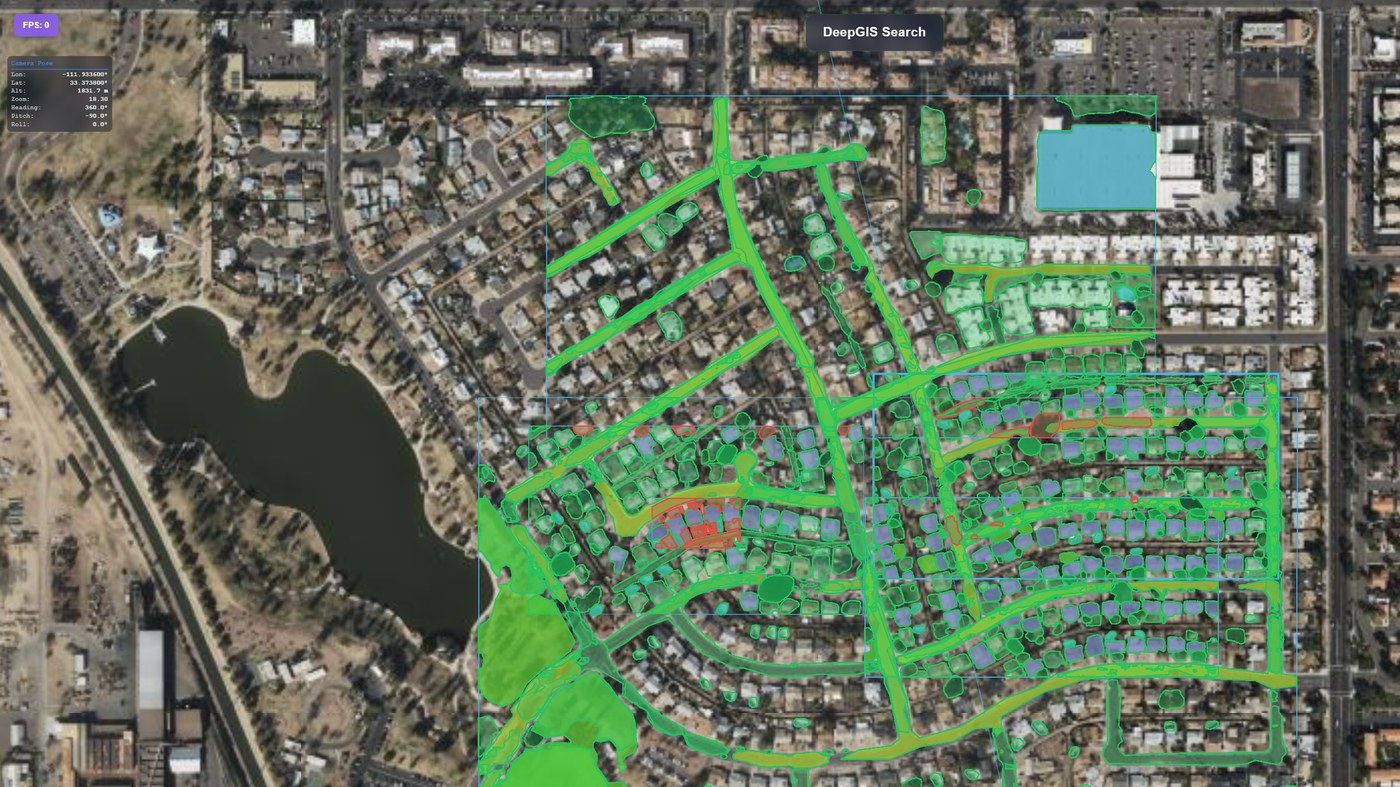
\includegraphics[width=\columnwidth]{world-changes-tempe.jpg}
\caption{``What changed here since June?'' over a Tempe neighbourhood: entities first seen since
1~June~2026 in green (973) and entities that later captures sharp enough to resolve them missed,
and that are now believed gone, in red (47). The blue outlines are capture footprints.}
\label{fig:changes}
\end{figure}

The world model is useful only if people can interrogate it. Five pilot actions do that.
\begin{itemize}
\item ``What's uncertain here?'' (\code{world\_uncertain}) counts the entities in view, the unknown
ones and what each most likely is, and how confidence is spread. At the Tempe test block: 332 of
1{,}073 objects are unknown, their best guesses mostly pavement (60), other vegetation (53) and
road (44), each at about 20\%.
\item ``Show only confident objects'' (\code{world\_confidence}) filters the layer by the top
category probability, 0.5 by default: 287 objects there.
\item \code{capture\_quality} (``How sharp were the captures here?'') lists each capture with its
GSD, the smallest object a miss can count for, $64\,\mathrm{GSD}^2$, and its pose uncertainty:
4.6\,cm to 21\,cm per pixel in November against 2.5\,m to 8.6\,m for the April captures.
\item ``What changed here since April?'' (\code{world\_changes}) draws entities first seen in the
window in green and entities missed in it and now believed gone ($p_{\text{exists}} < 0.5$) in red
(Fig.~\ref{fig:changes}). The prompt carries today's date so that ``since April'' resolves.
\item ``Remove that blob'' (\code{retire\_entity}, superusers) acts on the object the user clicked,
shows a confirm card, retires it and offers Undo.
\end{itemize}
With the default model, each of the five phrasings above produced exactly the intended action on
the first try. ``Remove that blob'' from a non-superuser cannot produce a retirement, because the
action is not in that user's schema and the server drops it.

%======================================================================
\section{Live Vehicles and Digital Twins}
\label{sec:robots}

Robots report pose and camera keyframes to the globe through token-authenticated endpoints. The
fleet includes Gazebo/PX4~\cite{meier2015,koenig2004} digital twins of a multirotor and a ground
rover at a fault-scarp site whose terrain is a photogrammetry mesh of the real place, a catamaran
surface vehicle on Tempe Town Lake, and a surface--underwater pair on Kiwanis Lake~\cite{coral2026},
plus students' OpenUAV~\cite{anand2019openuav} simulations and the lab's field rover. The pilot can
follow any of them through its own camera or from behind, describe what that camera sees, and,
for superusers, propose commands to the twins' mission supervisors over ROS~2~\cite{macenski2022}.

\emph{The field rover.} The rover spools telemetry locally and uploads it in gzip batches below
50\,kbit/s. It posts a 640$\times$480 keyframe every 10\,m, 30$^\circ$ or 30\,s, together with a
reduced spectrometer reading integrated across the frame and the laser range. Each reading is
stored in PostGIS with its camera point and, when heading and range are valid, the ground target.
It is annotated with sun geometry, the hour's weather and air quality, nearby aircraft, and two
vision-model notes: one on the photograph, one combining the photograph, the laser and the
spectrum. The server also advises the rover's spectrometer exposure. Rules derived from sun geometry
and motion give the advice; the language model may adjust it, but only toward caution while the
rover moves, and the per-reading exposure loop stays on the rover. More than 2{,}400 readings were
stored in the first week.

\emph{Twins from the globe.} \code{create\_twin} turns the view into a simulation. The page samples
a 65$\times$65 grid of the globe's own terrain around the crosshair; the builder writes it as a
Gazebo heightmap, drapes a public satellite image of the patch, raises OpenStreetMap building
footprints by their height or levels, adds props from a vision model's reading of the nadir frame,
and spawns a camera multirotor that reports back to the same globe. On the Moon the same path uses
the lunar elevation model. Each session gets its own simulator, ROS domain and desktop port, and
its owner can stop, start and purge it.

%======================================================================
\section{Immersive Cockpit}
\label{sec:vr}

\begin{figure}[t]
\centering
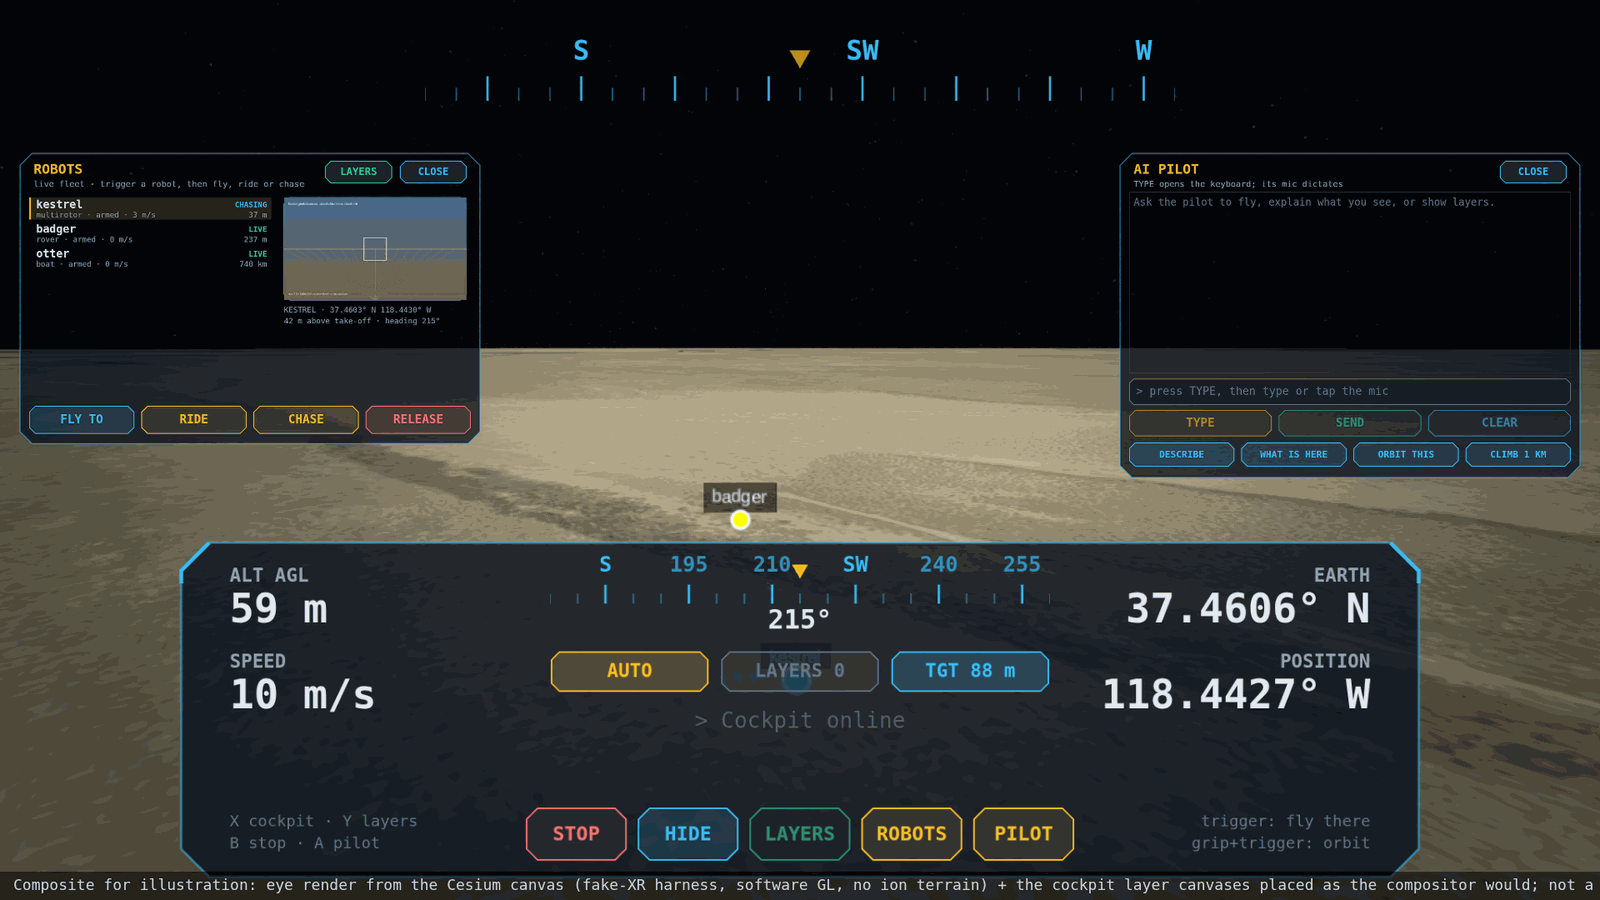
\includegraphics[width=\columnwidth]{vr-headset-view-composite.png}
\caption{The WebXR cockpit: a console cylinder with altitude, speed, heading tape and controls,
side panels for layers and the pilot's chat, a wrist menu, and the globe rendered per eye.}
\label{fig:vr}
\end{figure}

CesiumJS~1.111 has no WebXR support, so the cockpit renders the globe once per eye with a
symmetric frustum and copies each image into a WebXR projection layer. A rig maps the headset's
local space to east--north--up coordinates on the globe, and Cesium's own render loop and mouse
controls are suspended for the session. The panels are WebXR compositor layers drawn on 2D canvases
(Fig.~\ref{fig:vr}): a console, a head-locked compass, layer and chat panels at $\pm 50^\circ$, a
robots panel with live camera frames, and a wrist menu. The left stick flies along the craft's
heading with eased acceleration. The right stick snap-turns and climbs. The trigger flies to the
ground point under the laser, or orbits it. A comfort vignette follows optic flow. The pilot works
inside the session, including the Quest system keyboard. The cockpit has been verified with a
scripted fake-XR harness that captures every panel and checks motion against the rig, but not yet
on a physical headset.

%======================================================================
\section{Engineering Practice}
\label{sec:practice}

DeepGIS is built and operated by a small lab, increasingly with AI coding agents working in
parallel sessions on one live checkout. Four practices keep that safe.
\begin{enumerate}
\item \emph{Deploy is copy, lint, version, reload.} Static scripts are syntax-checked before
deployment, cache-busted by a version tag in both page templates, and the application server
reloads gracefully.
\item \emph{Never erase; supersede.} The rule the world model follows applies to the project's own
records: the architecture document is dated, and later sections supersede earlier ones without
deleting them.
\item \emph{Public and private are separate.} The open-source repository holds no network
addresses, topology or tokens; those live in a private infrastructure repository. Diffs are scanned
for addresses before every commit, and secret-bearing files are never staged.
\item \emph{Reconcile before committing.} Several sessions' uncommitted work can sit in one tree.
Each session reads the others' diffs before committing them, the development analogue of
associating a detection with an entity.
\end{enumerate}

%======================================================================
\section{Limitations and Future Work}
\label{sec:limits}

\emph{The learning loop is still open.} The system has become much better at seeing and remembering
than at learning from what it remembers. No model is retrained on stored labels, no detector's
accuracy is logged, and the feedback table that would recalibrate each source's confusion table
has no rows yet. The world model's confidences are therefore not calibrated; the unknown label and
the geometry priors make that visible rather than solve it. The next steps are, in order, a small
ground-truth set to measure the world model's accuracy, a labelling session that starts the
feedback refit, and automatic ingest from the rover.

\emph{Known data issues.} The 16{,}749 April entities with projected coordinates need reprojection;
the map adapter appears to clip roads to the capture frame; and the public map query service is too
slow for interactive builds without a cache.

\emph{Toward Kimera at the vehicle scale.} The store already anchors evidence to capture poses
with uncertainty. The plan is to add a zone layer above objects with partitioned inference, an
offline rover pipeline that turns recorded drives into pose-graph keyframes with segmented
landmarks, calibration of the aerial sources against the rover's ground truth, re-derivation of
evidence when a pose is optimised, and a landmark subgraph that a rover takes into the field.

\emph{Evaluation.} The results in this report are single runs on the live system or in
simulation. The pilot's mapping from sentences to actions, the world model's change detection and
the cockpit's comfort all need repeated trials and user studies.

%======================================================================
\section{Conclusion}
\label{sec:conclusion}

DeepGIS makes a geospatial platform, a detector bench, a robot ground station, a twin builder and a
world model answer to the same sentences. The language model plans and the server constrains it.
The person confirms anything with consequences. The memory supersedes instead of erasing, and says
when it does not know. The next phase is less about seeing more and more about knowing what the
system knows: making its confidences mean something, and closing the loop back to the robots.

\section*{Acknowledgments}
The author thanks the DREAMS Lab and Earth Innovation Hub members whose field data, simulations
and code this system builds on, and the providers of the open data and models it uses, including
Cesium, USGS, NASA, ESA Copernicus, Macrostrat, OpenStreetMap and OpenTopography.

\begin{thebibliography}{99}

\bibitem{das2015ijrr}
J.~Das \emph{et~al.}, ``Data-driven robotic sampling for marine ecosystem monitoring,''
\emph{Int.\ J.\ Robot.\ Res.}, vol.~34, no.~12, 2015, doi: 10.1177/0278364915587723.

\bibitem{chen2020iros}
Z.~Chen \emph{et~al.}, ``Geomorphological analysis using unpiloted aircraft systems, structure
from motion, and deep learning,'' in \emph{Proc.\ IEEE/RSJ Int.\ Conf.\ Intell.\ Robots Syst.\
(IROS)}, 2020, doi: 10.1109/IROS45743.2020.9341354.

\bibitem{chen2023espl}
Z.~Chen, C.~Scott, D.~Keating, A.~Clarke, J.~Das, and R.~Arrowsmith, ``Quantifying and analysing
rock trait distributions of rocky fault scarps using deep learning,'' \emph{Earth Surf.\ Process.\
Landforms}, vol.~48, no.~6, 2023, doi: 10.1002/esp.5545.

\bibitem{anand2019openuav}
H.~Anand \emph{et~al.}, ``{OpenUAV} cloud testbed: A collaborative design studio for field
robotics,'' in \emph{Proc.\ IEEE Int.\ Conf.\ Autom.\ Sci.\ Eng.\ (CASE)}, 2021,
doi: 10.1109/CASE49439.2021.9551638.

\bibitem{coral2026}
J.~Das, ``{CoRAL}: Language-specified joint missions of an autonomous surface vehicle and an
autonomous underwater vehicle,'' preprint, 2026. [Online]. Available:
\url{https://github.com/Earth-Innovation-Hub/coral}

\bibitem{cesium}
Cesium GS, ``{CesiumJS}: 3D geospatial visualization for the web.'' [Online]. Available:
\url{https://cesium.com/platform/cesiumjs/}

\bibitem{kirillov2023sam}
A.~Kirillov \emph{et~al.}, ``Segment anything,'' in \emph{Proc.\ IEEE/CVF Int.\ Conf.\ Comput.\
Vis.\ (ICCV)}, 2023, pp.~4015--4026.

\bibitem{carion2025sam3}
N.~Carion \emph{et~al.}, ``{SAM}~3: Segment anything with concepts,'' arXiv preprint, 2025.

\bibitem{liu2024gdino}
S.~Liu \emph{et~al.}, ``Grounding {DINO}: Marrying {DINO} with grounded pre-training for open-set
object detection,'' in \emph{Proc.\ Eur.\ Conf.\ Comput.\ Vis.\ (ECCV)}, 2024.

\bibitem{he2017maskrcnn}
K.~He, G.~Gkioxari, P.~Doll\'ar, and R.~Girshick, ``Mask {R-CNN},'' in \emph{Proc.\ IEEE Int.\
Conf.\ Comput.\ Vis.\ (ICCV)}, 2017, pp.~2961--2969.

\bibitem{ultralytics}
G.~Jocher, J.~Qiu, and A.~Chaurasia, ``Ultralytics {YOLO},'' software. [Online]. Available:
\url{https://github.com/ultralytics/ultralytics}

\bibitem{armeni2019sg}
I.~Armeni, Z.-Y. He, J.~Gwak, A.~R. Zamir, M.~Fischer, J.~Malik, and S.~Savarese, ``{3D} scene
graph: A structure for unified semantics, {3D} space, and camera,'' in \emph{Proc.\ IEEE/CVF Int.\
Conf.\ Comput.\ Vis.\ (ICCV)}, 2019, pp.~5664--5673.

\bibitem{rosinol2021kimera}
A.~Rosinol, A.~Violette, M.~Abate, N.~Hughes, Y.~Chang, J.~Shi, A.~Gupta, and L.~Carlone,
``Kimera: From {SLAM} to spatial perception with {3D} dynamic scene graphs,'' \emph{Int.\ J.\
Robot.\ Res.}, vol.~40, no.~12--14, pp.~1510--1546, 2021.

\bibitem{hughes2022hydra}
N.~Hughes, Y.~Chang, and L.~Carlone, ``Hydra: A real-time spatial perception system for {3D}
scene graph construction and optimization,'' in \emph{Proc.\ Robot.:\ Sci.\ Syst.\ (RSS)}, 2022.

\bibitem{kschischang2001}
F.~R. Kschischang, B.~J. Frey, and H.-A. Loeliger, ``Factor graphs and the sum-product
algorithm,'' \emph{IEEE Trans.\ Inf.\ Theory}, vol.~47, no.~2, pp.~498--519, 2001.

\bibitem{dellaert2017}
F.~Dellaert and M.~Kaess, ``Factor graphs for robot perception,'' \emph{Found.\ Trends Robot.},
vol.~6, no.~1--2, pp.~1--139, 2017.

\bibitem{murphy1999loopy}
K.~P. Murphy, Y.~Weiss, and M.~I. Jordan, ``Loopy belief propagation for approximate inference:
An empirical study,'' in \emph{Proc.\ Conf.\ Uncertainty Artif.\ Intell.\ (UAI)}, 1999,
pp.~467--475.

\bibitem{moravec1985}
H.~Moravec and A.~Elfes, ``High resolution maps from wide angle sonar,'' in \emph{Proc.\ IEEE
Int.\ Conf.\ Robot.\ Autom.\ (ICRA)}, 1985, pp.~116--121.

\bibitem{snodgrass1999}
R.~T. Snodgrass, \emph{Developing Time-Oriented Database Applications in {SQL}}. San Francisco,
CA, USA: Morgan Kaufmann, 1999.

\bibitem{kernelcal}
Earth Innovation Hub, ``kernelcal: Calibrated fusion of perception kernels,'' software, 2026.

\bibitem{ahn2022saycan}
M.~Ahn \emph{et~al.}, ``Do as {I} can, not as {I} say: Grounding language in robotic
affordances,'' in \emph{Proc.\ Conf.\ Robot Learn.\ (CoRL)}, 2022.

\bibitem{liang2023cap}
J.~Liang, W.~Huang, F.~Xia, P.~Xu, K.~Hausman, B.~Ichter, P.~Florence, and A.~Zeng, ``Code as
policies: Language model programs for embodied control,'' in \emph{Proc.\ IEEE Int.\ Conf.\
Robot.\ Autom.\ (ICRA)}, 2023, pp.~9493--9500.

\bibitem{mcp2024}
Anthropic, ``Model Context Protocol specification,'' 2024. [Online]. Available:
\url{https://modelcontextprotocol.io}

\bibitem{meier2015}
L.~Meier, D.~Honegger, and M.~Pollefeys, ``{PX4}: A node-based multithreaded open source robotics
framework for deeply embedded platforms,'' in \emph{Proc.\ IEEE Int.\ Conf.\ Robot.\ Autom.\
(ICRA)}, 2015, pp.~6235--6240.

\bibitem{koenig2004}
N.~Koenig and A.~Howard, ``Design and use paradigms for {Gazebo}, an open-source multi-robot
simulator,'' in \emph{Proc.\ IEEE/RSJ Int.\ Conf.\ Intell.\ Robots Syst.\ (IROS)}, 2004,
pp.~2149--2154.

\bibitem{macenski2022}
S.~Macenski, T.~Foote, B.~Gerkey, C.~Lalancette, and W.~Woodall, ``Robot {Operating System 2}:
Design, architecture, and uses in the wild,'' \emph{Sci.\ Robot.}, vol.~7, no.~66, p.~eabm6074,
2022.

\end{thebibliography}

\end{document}
